\documentclass[tc, manuscript]{copernicus}

%\usepackage{xr}
%\usepackage{hyperref}
%\usepackage{appendix}

% check if we are compiling under latex or pdflatex
%\ifx\pdftexversion\undefined
%\usepackage[dvips]{graphicx}
%\else
%\usepackage[pdftex]{graphicx}
%\usepackage{epstopdf}
%\epstopdfsetup{suffix=}
%\fi

% the default is for unnumbered section heads
% if you really must have numbered sections, remove
% the % from the beginning of the following command
% and insert the level of sections you wish to be
% numbered (up to 4):

% \setcounter{secnumdepth}{2}

\begin{document}
\title{\textit{Supplement} of ``Diagnosing the sensitivity of grounding line flux to changes in sub-ice shelf melting''}

\Author[1]{Tong}{Zhang}
\Author[1]{Stephen}{Price}
\Author[1]{Matthew}{Hoffman}
\Author[2]{Mauro}{Perego}
\Author[1]{Xylar}{Asay-Davis}

\affil[1]{Fluid Dynamics and Solid Mechanics Group, Los Alamos National Laboratory, Los Alamos, NM, 87545, USA}
\affil[2]{Center for Computing Research, Sandia National Laboratories, Albuquerque, NM, 87185, USA}

\runningtitle{Diagnosising the sensitivity of grounding line flux to sub-ice shelf melting}
\runningauthor{T.~Zhang et al.}
\correspondence{T.~Zhang (tzhang@lanl.gov)}

\received{}
\pubdiscuss{} %% only important for two-stage journals
\revised{}
\accepted{}
\published{}

\firstpage{1}
\maketitle


\section{Appendix materials}
%\renewcommand\thefigure{\thesection.\arabic{figure}}  
\renewcommand{\thefigure}{A\arabic{figure}}
\setcounter{figure}{0}

\begin{figure}
\centering
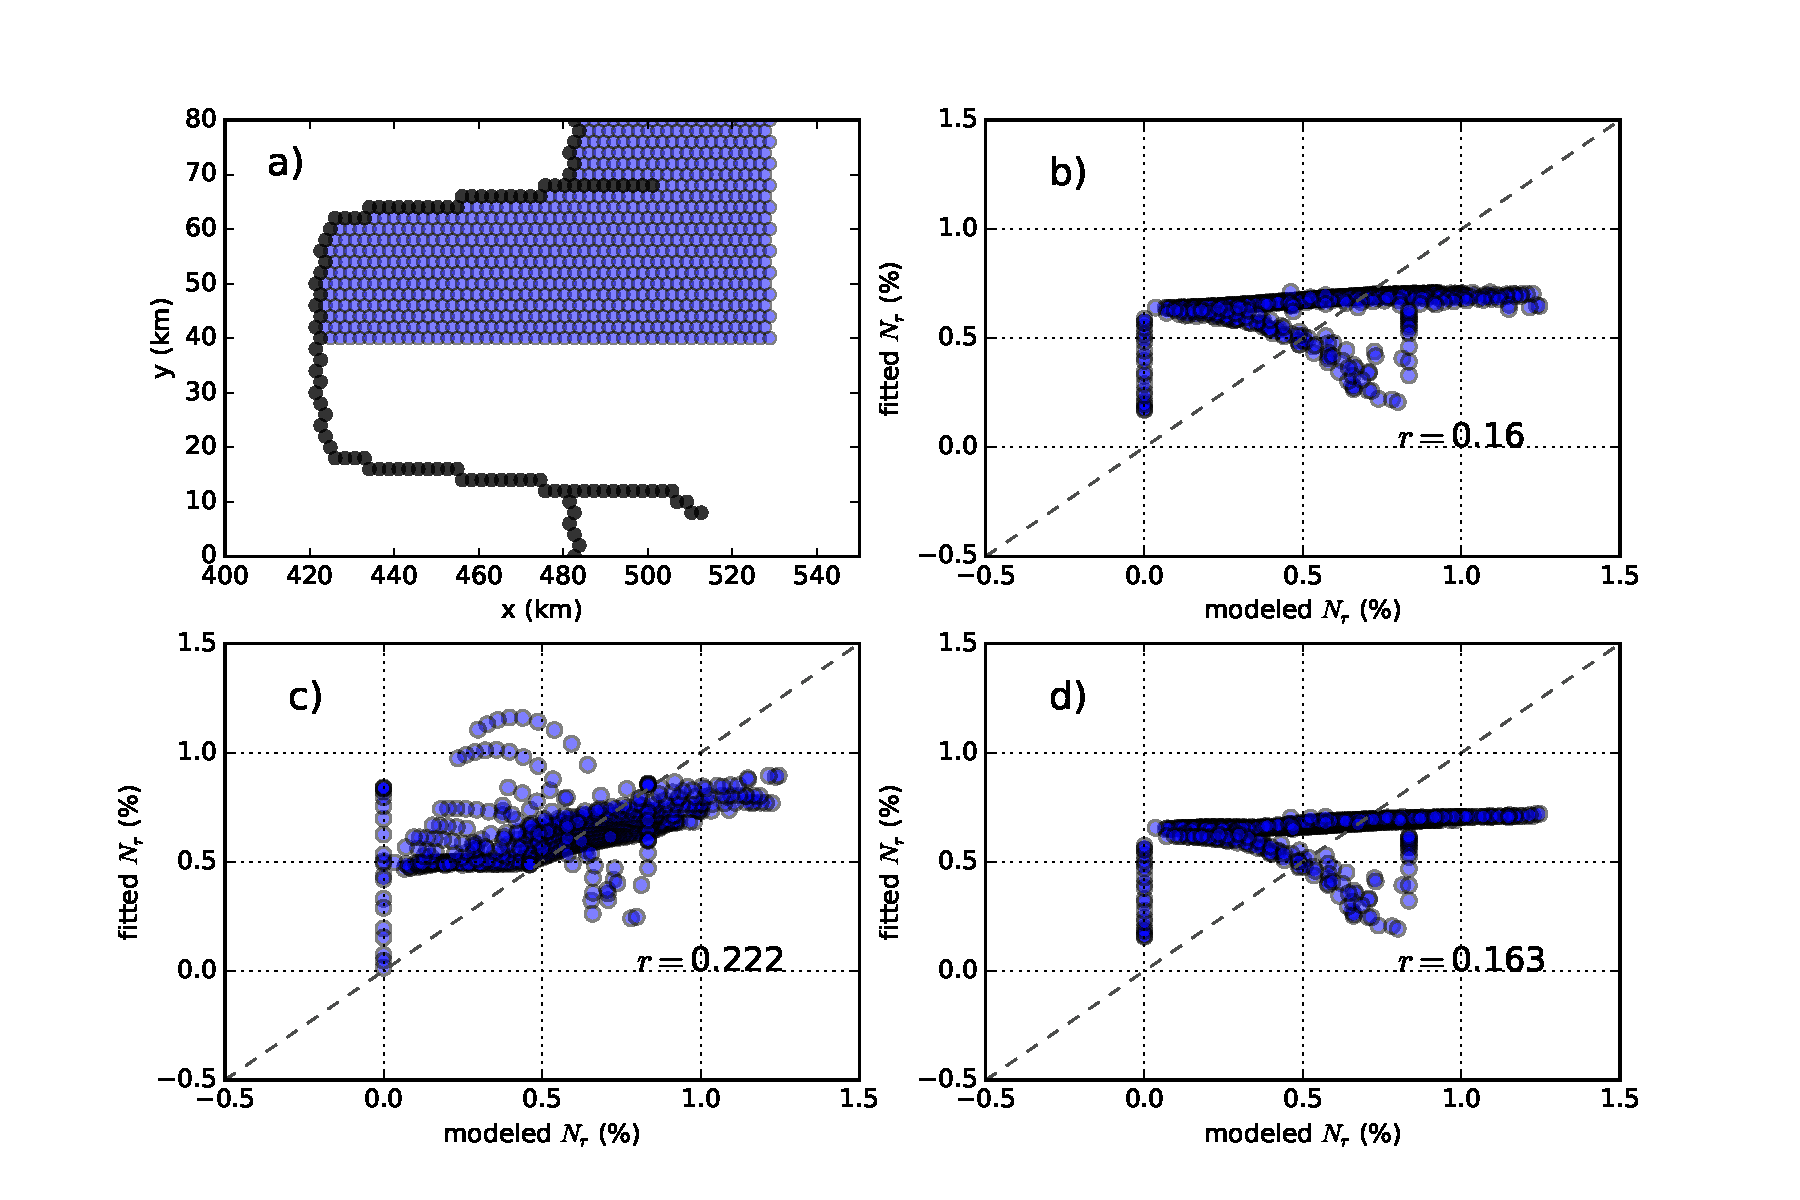
\includegraphics[width=1\linewidth]{./figs/mismip_Nb_GLF_regression_all_points.pdf}
    \caption{(a) Blue dots are all perturbation points for $N_r\left(N_b\right)$ linear regression analysis and the black dots represent grid cells along the grounding line. (b) Modeled $N_r$ from perturbation experiments versus fitted $N_r$ as a function of $N_b$ that is calculated along $\textbf{n}_{p1}$; (c) Modeled $N_r$ from perturbation experiments versus fitted $N_r$ as a function of $N_b$ that is calculated along $\textbf{n}_{p2}$; (d) Modeled $N_r$ from perturbation experiments versus fitted $N_r$ as a function of $N_b$ that is calculated along $\textbf{n}_{f}$. $r$ is the correlation coefficient. \textbf{Tong: Do we need to include the information of significant level along with correlation coefficient?}}
\label{mismip_Nb_GLF_regression_all_points}
\end{figure}

%\begin{figure}
%	\centering
%	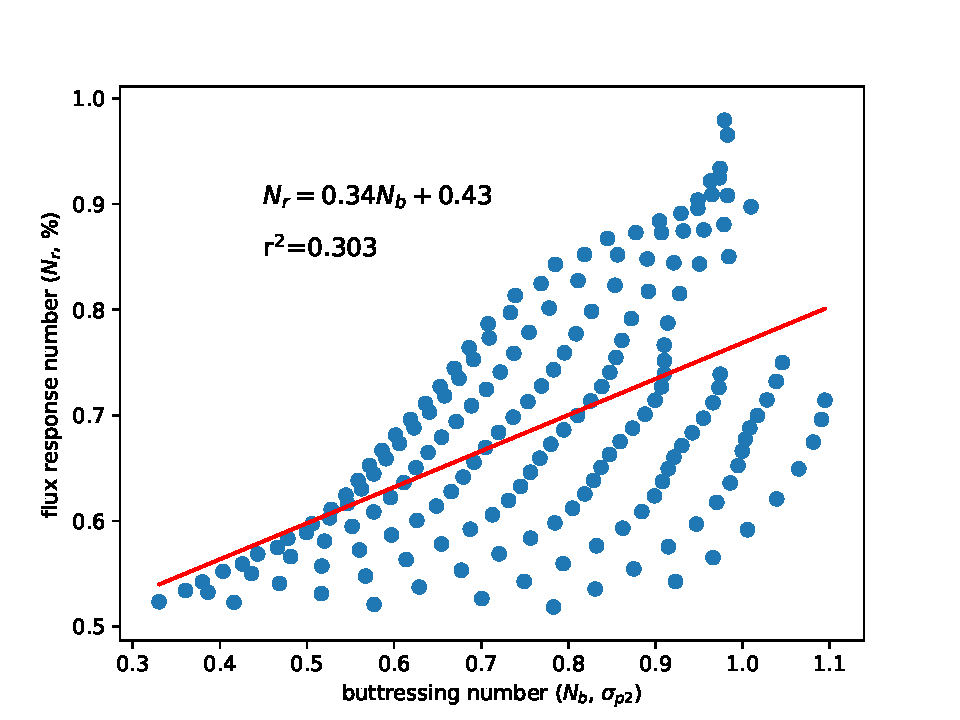
\includegraphics[width=1\linewidth]{figs/sigma_p2_example.pdf}
%	\caption{$N_b$:$N_r$ correlation for perturbation points within the confined region of the shelf and with a thickness gradient magnitude $\left|\nabla H\right|<7$x$10^{-3}$. $N_b$ is calculated from the second principal stress $\sigma_{p2}$.}
%	\label{sigma_p2_example}
%\end{figure}

\begin{figure}
	\centering
	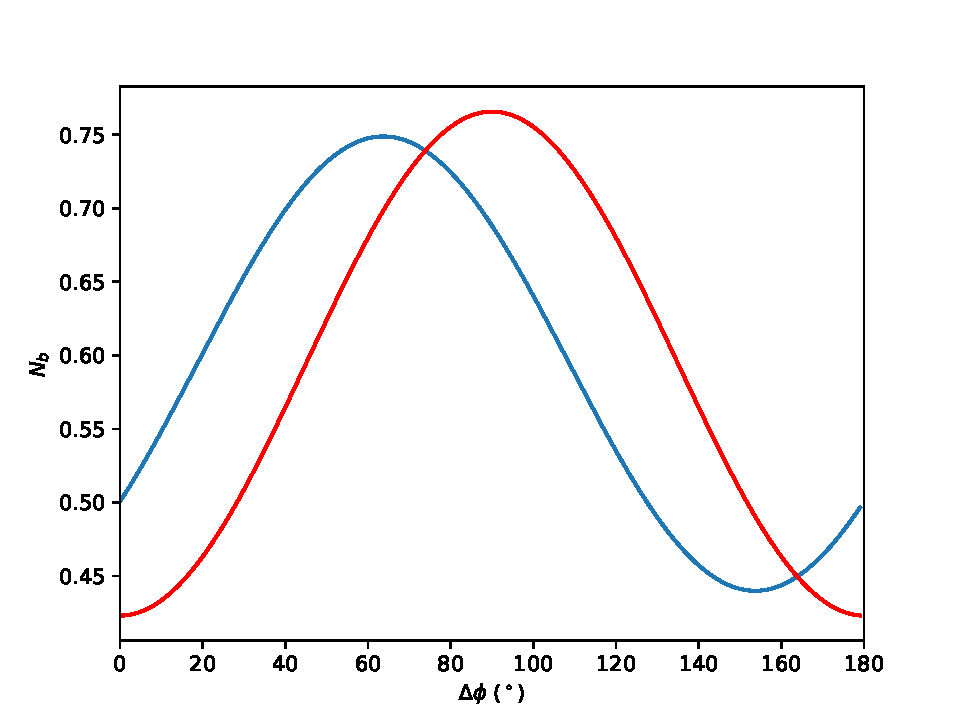
\includegraphics[width=1\linewidth]{./figs/Nb_Deltaphi.pdf}
	\caption{(a) $N_b$ values rotated counterclockwise by $\Delta\phi$ degrees relative to the direction corresponding to $\sigma_{p1}$ ($\mathbf{n}_{p1}$); (b) $N_b$ values rotated counterclockwise by $\Delta\phi$ degrees relative to the direction corresponding to $\sigma_{p1}$ ($\mathbf{n}_{f}$). Note that these are mean $N_b$ values for those perturbation points shown in Fig.~\ref{mismip_Nb_GLF_regression}a. It's a twin plot for Fig.~\ref{mismip_Nb_GLF_regression}a and b. Both curves show the buttressing number is largest along the direction corresponding to $\sigma_{p2}$ ($\mathbf{n}_{p2}$), i.e., in (a) $N_b$ is the largest when $\Delta\phi\approx 90^\circ$ relative to $\mathbf{n}_{p1}$, and in (b) $N_b$ is the largest when $\Delta\phi\approx 62^\circ$ relative to $\mathbf{n}_{f}$ which is $\Delta\phi+\Delta\varphi$ (around 92--102$^\circ$) relative to $\mathbf{n}_{p1}$ ($\Delta\varphi$ is the angle difference between $\mathbf{n}_{f}$ and $\mathbf{n}_{p1}$, around 30--50$^\circ$; see Section~\ref{directional_buttressing}).}
	\label{Nb_Deltaphi}
\end{figure}

\begin{figure}
	\centering
	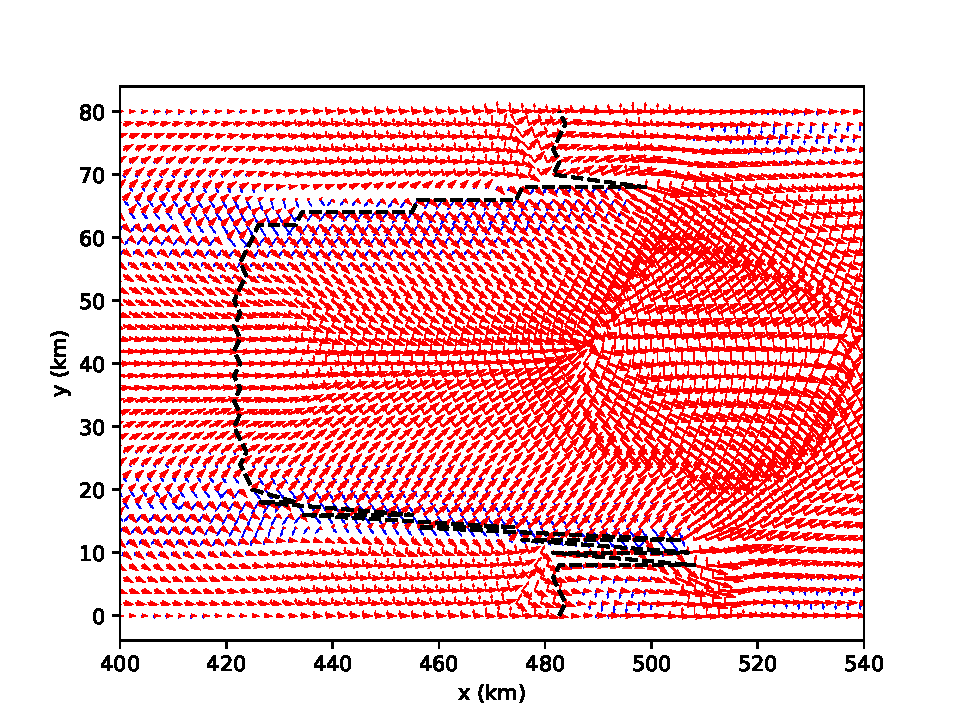
\includegraphics[width=1\linewidth]{figs/principal_stress_quiver.pdf}
	\caption{The quiver plot of $\sigma_{p1}$ (thick arrows) and $\sigma_{p2}$ (thin arrows) field. The red and blue colors means tensile and compressive stress, respectively. The thick dashed black line represents the grounding line.}
	\label{principal_stress_quiver}
\end{figure}

\begin{figure}
 	\centering
     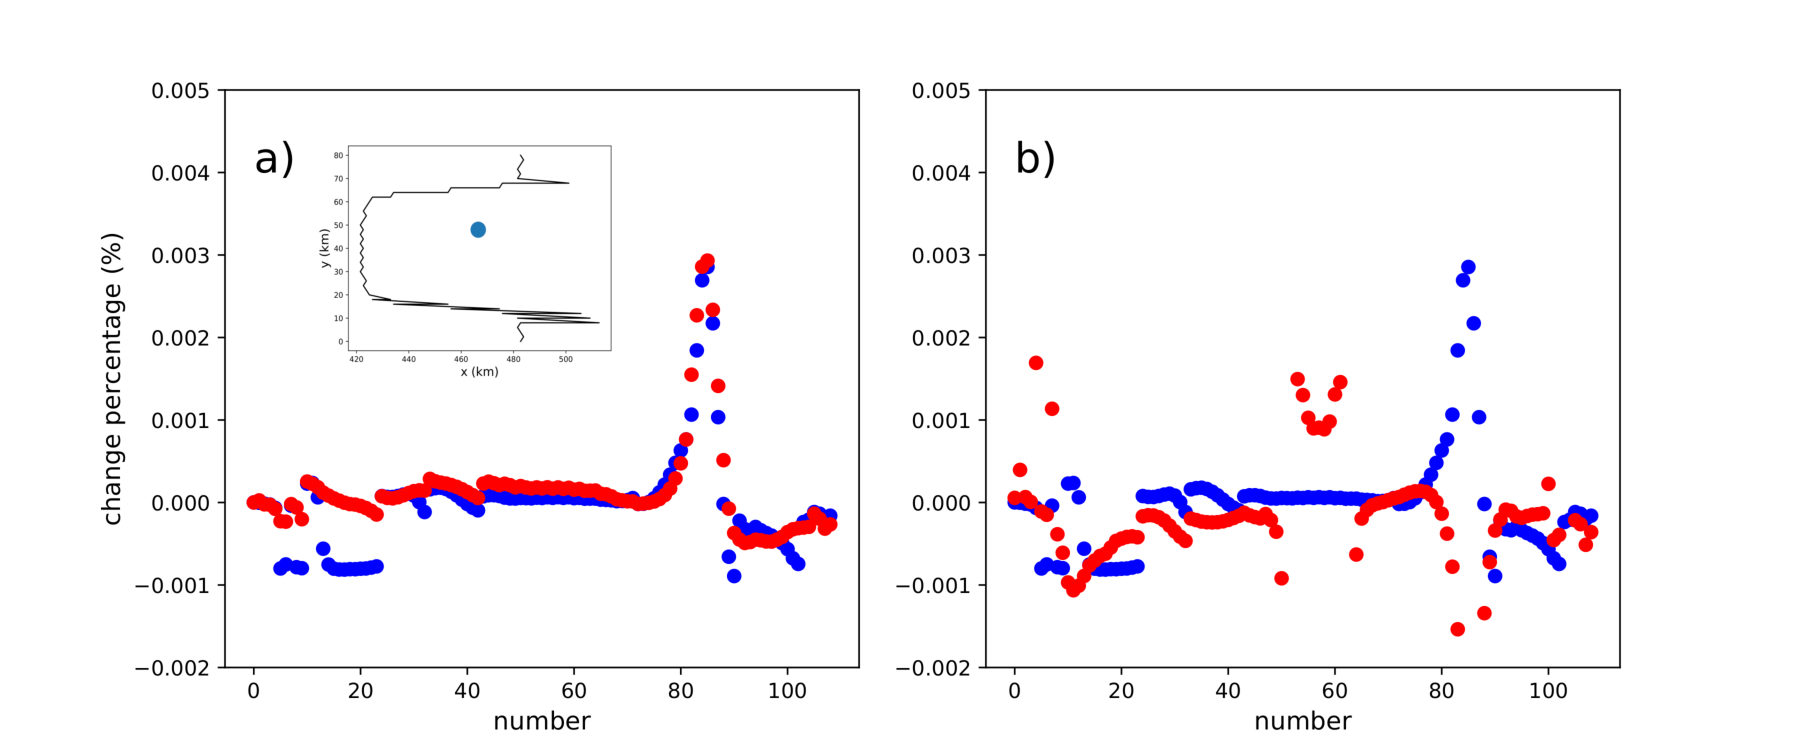
\includegraphics[width=1\linewidth]{figs/vel_stress_change_example.pdf}
     \caption{Relationship between changes in velocity (blue) and changes in the stress (red) along the GL for the MISMIP+ test case, due to a perturbation at a specific location on the ice shelf (blue dot in inset map). In a), changes in GL velocities are plotted against changes in $\sigma_{p1}$. In b), changes in GL velocity are plotted against changes in $\sigma_{p2}$. The $x$-axis represents an index for the grid cell number along the GL.}
 	\label{vel_stress_change_example}
\end{figure}

\begin{figure}
	\centering
	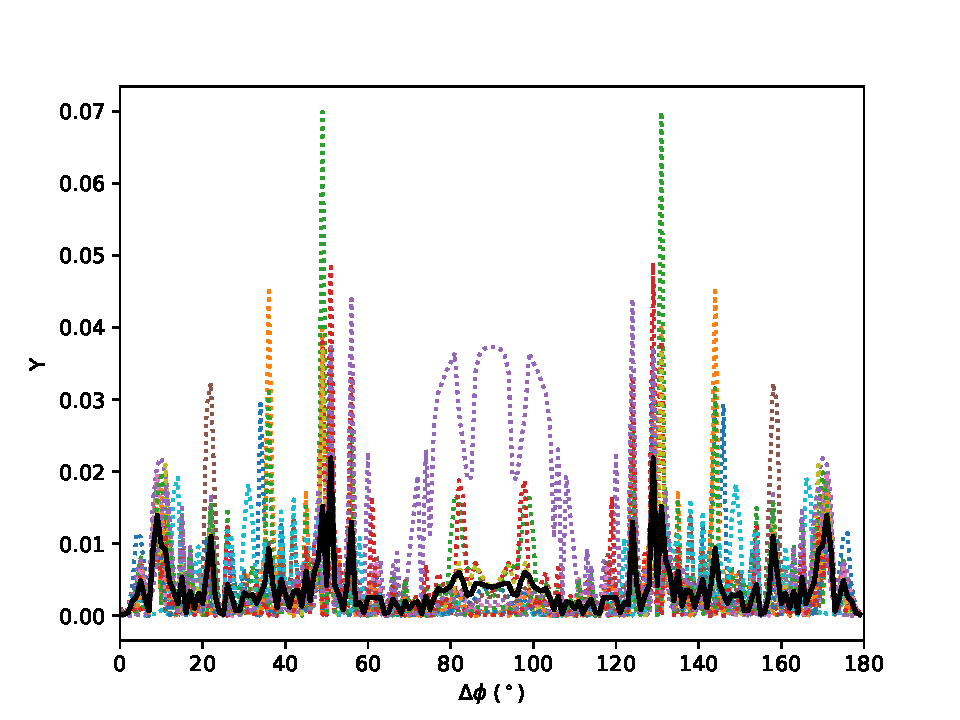
\includegraphics[width=1\linewidth]{figs/stress_vel_corr_GL_allP_larsenC.pdf}
	\caption{The correlation ($\Upsilon$) between the changes of ice surface speed and the changes of normal stress along GL for the Larsen C experiments. The direction of normal stress is rotated counterclockwise from the direction of $\sigma_{p1}$. The colored dashed curve each represents a perturbation experiment, and the thick back curve is their mean value.}
	\label{stress_vel_corr_GL_allP_larsenC}
\end{figure}

\begin{figure}
	\centering
    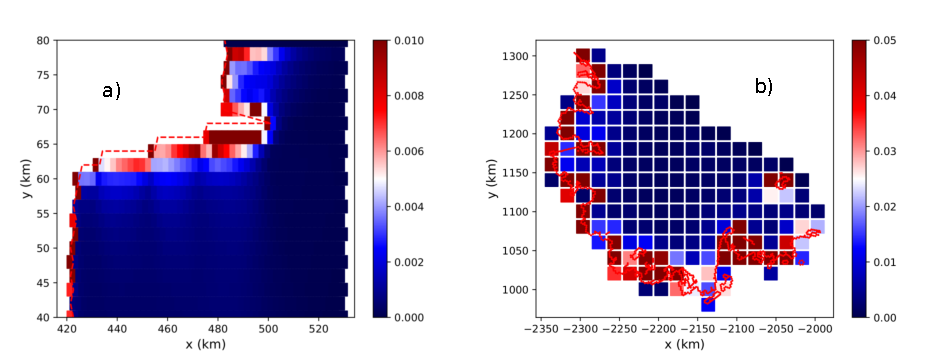
\includegraphics[width=1\linewidth]{figs/vel_change_std.pdf}
    \caption{Standard deviation of velocity change along GL for each perturbation point for the MISMIP+ (a) and Larsen C (b) experiment. The red dashed lines (points) are the GLs for MISMIP+ (a) and Larsen C (b) .}
	\label{vel_change_std}
\end{figure}


\begin{figure}
	\centering
	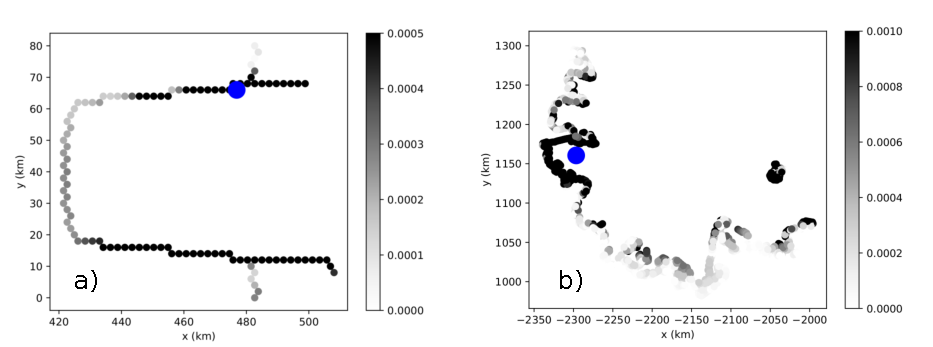
\includegraphics[width=1\linewidth]{figs/mismip_larsenC_velChange.pdf}
	\caption{The ice surface speed change (\%) along grounding line under certain specified perturbation locations for MISMIP+ (a) and Larsen C (b).}
	\label{mismip_larsenC_velChange}
\end{figure}

\begin{figure}
	\centering
    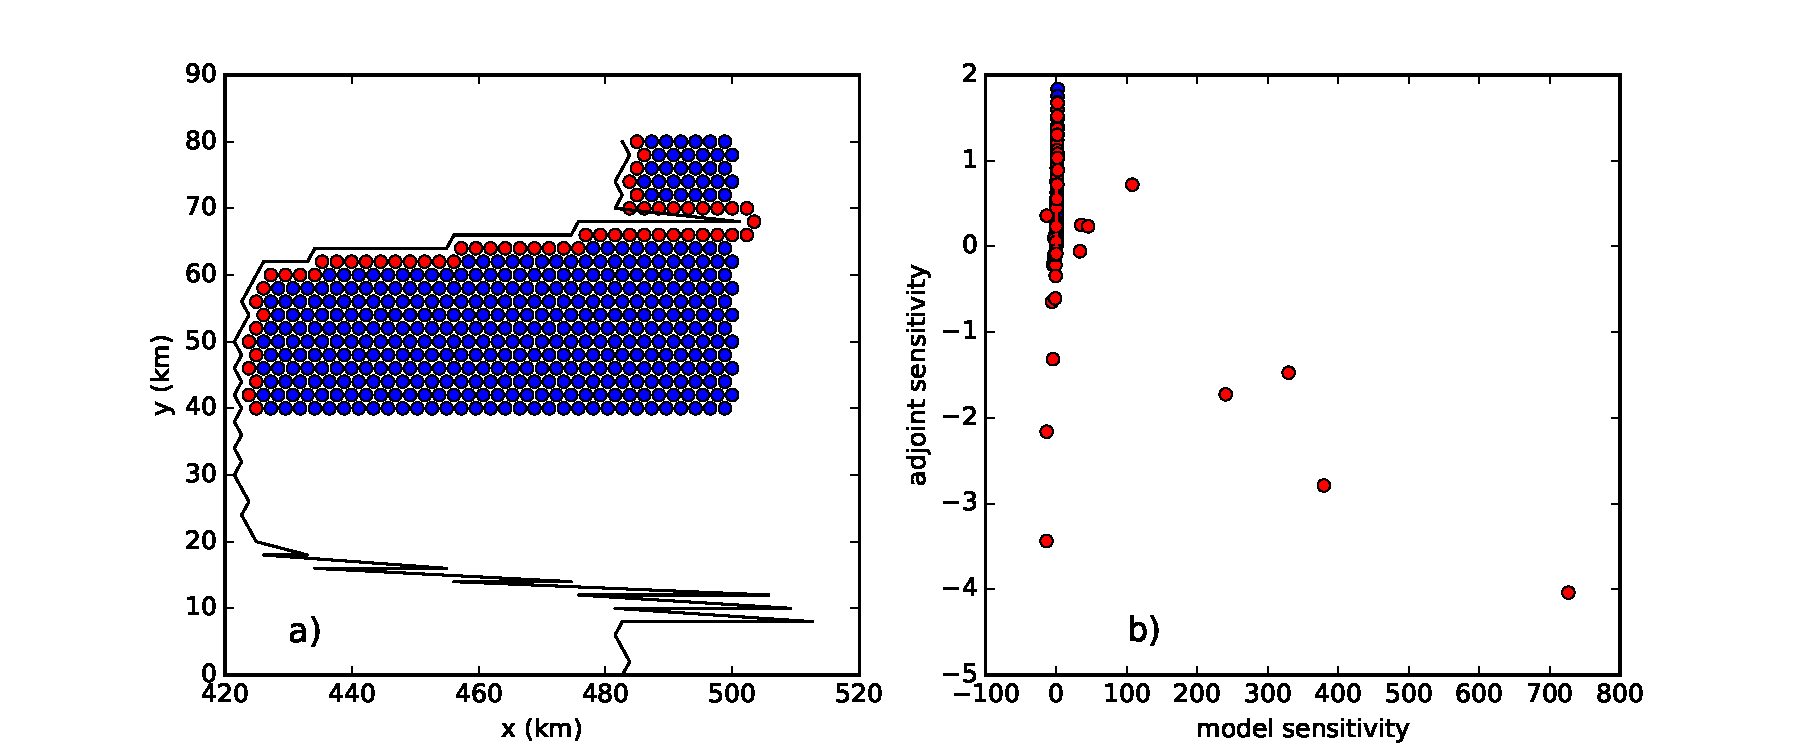
\includegraphics[width=1\linewidth]{figs/adjoint_comp_appendix.pdf}
    \caption{Grounding line flux sensitivity for the MISMIP+ domain calculated from individual perturbation experiments versus derived from a model adjoint (perturbation locations are shown by circles in a). Perturbation-experiment (x-axis) and adjoint-derived (y-axis) sensitivities (see text for definition) are plotted against one another in b). In a and b, the red circles indicate near-GL ($<$2 km) perturbation points, which are omitted in the comparison in Fig.~\ref{adjoint_comp}. The GL in a) is shown by the black curve. In b), the red line is a linear regression between the perturbation-experiment and adjoint-derived sensitivities.}
	\label{adjoint_comp_appendix}
\end{figure}

\subsection{A metric connecting perturbations in thickness to changes in GLF} \label{new_metric}
%\textbf{SP: I think we might want to copy/paste this whole section into the appendix for the time being. In some of the discussion with Xylar and Matt, we decided this does not necessarily add any new information that we don't already know from other calculations above (e.g., it uses/needs a lot of the same information that we currently show in fig 3 above) but it is much harder to understand. At this point, I think we know we aren't going to find a better simple metric than just the buttressing number using the p1 direction, so it doesn't make sense to try to introduce a more complicated one (and we're going to advocate for the adjoint approach in the end anyway).}
The change in GLF for a given perturbation to the ice-shelf thickness must be controlled by both the perturbation itself (the local change to the geometry, stress, and velocity fields) and the broader, surrounding ice dynamical setting (the regional geometry, stress, and velocity fields). To explore this further, we propose the following simplified metric, which connects and combines local aspects of a perturbation with its regional impact on GLF:
\begin{equation}
    \Lambda = \sum_i^I \frac{1}{d_i} |\mathrm{cos} \left(\theta_i\right)|,
    \label{Lambda}
\end{equation}
where $I$ is the total number of grid cells along the GL, $d_i$ is the distance between the perturbation point and the $i$-th GL grid cell, and $\theta_i$ is the angular difference between the direction of the specified normal stress (e.g., $\sigma_{p1}$) at the perturbation point and the flow direction for the $i$-th GL grid cell. The metric $\Lambda$ thus aims to capture two important factors impacting changes in GLF as a function of perturbations in ice shelf thickness: 1) the distance between the perturbation point and the GL (intuitively, the closer the perturbation to the GL, the larger the impact---also see the related discussion in the next section). We note that, while this metric does not \textit{explicitly} account for kinematic or dynamical processes (i.e., there are no terms explicitly involving velocities or stresses), it accounts for them \textit{implicitly} through the term in the numerator, which requires knowledge of the velocity and stress directions. 

Similar to above, we rotate the buttressing direction by 0--180$^\circ$ with respect to $\mathbf{n}_{p1}$, and calculate $\Lambda$ for each perturbation point. From Fig.~\ref{new_metric_new} we can see that $\Lambda$ has large values when the buttressing directions are close to $\mathbf{n}_{p1}$ ($\Delta\phi=0^\circ$ or $\Delta\phi=180^\circ$). A possible reason is that, for the MISMIP+ geometry, the velocity across the GL (and thus the GLF) is largely parallel with the $\sigma_{p1}$ direction at the GL (see Fig.~\ref{principal_stress_quiver}). This, in turn, is largely the result of extensional flow across the majority of the MISMIP+ GL.
%For grid cells where $\sigma_{p2}$ is also important, we can also see good matches between the changes of velocity and $\sigma_{p2}$ on GL, for example, grid cell number 65--75 and 90--95 in Fig.~\ref{vel_stress_change_example}b. 
For real ice shelves, where the pattern of ice flow across the GL is generally more complex (e.g., in the presence of an ice rise downstream from the GL), we expect a metric based on the assumption that $\sigma_{p1}$ and changes in GLF are well correlated to be less robust
.  


\begin{figure}
	\centering
    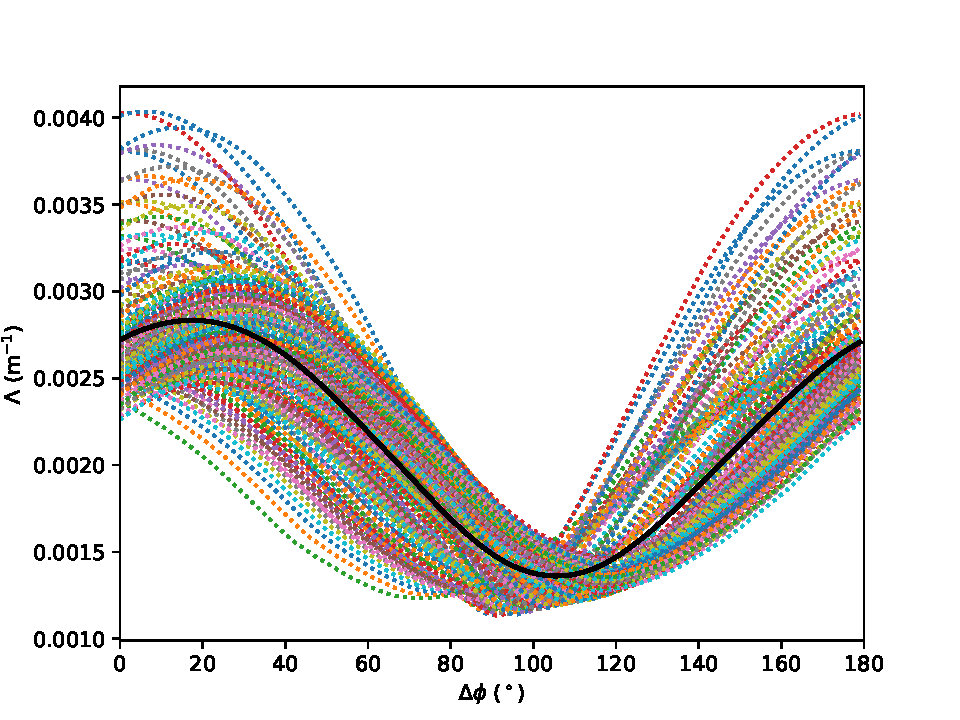
\includegraphics[width=1\linewidth]{figs/new_metric_new.pdf}
    \caption{A metric that gives a possible explanation of the connection between perturbation and GLF. Same as above, $\Delta\phi$ is the angular distance from the direction of $\sigma_{p1}$. The line types are the same as in Fig.~\ref{stress_vel_corr_GL_allP}}
	\label{new_metric_new}
\end{figure}


%\begin{figure}
%	\centering
%	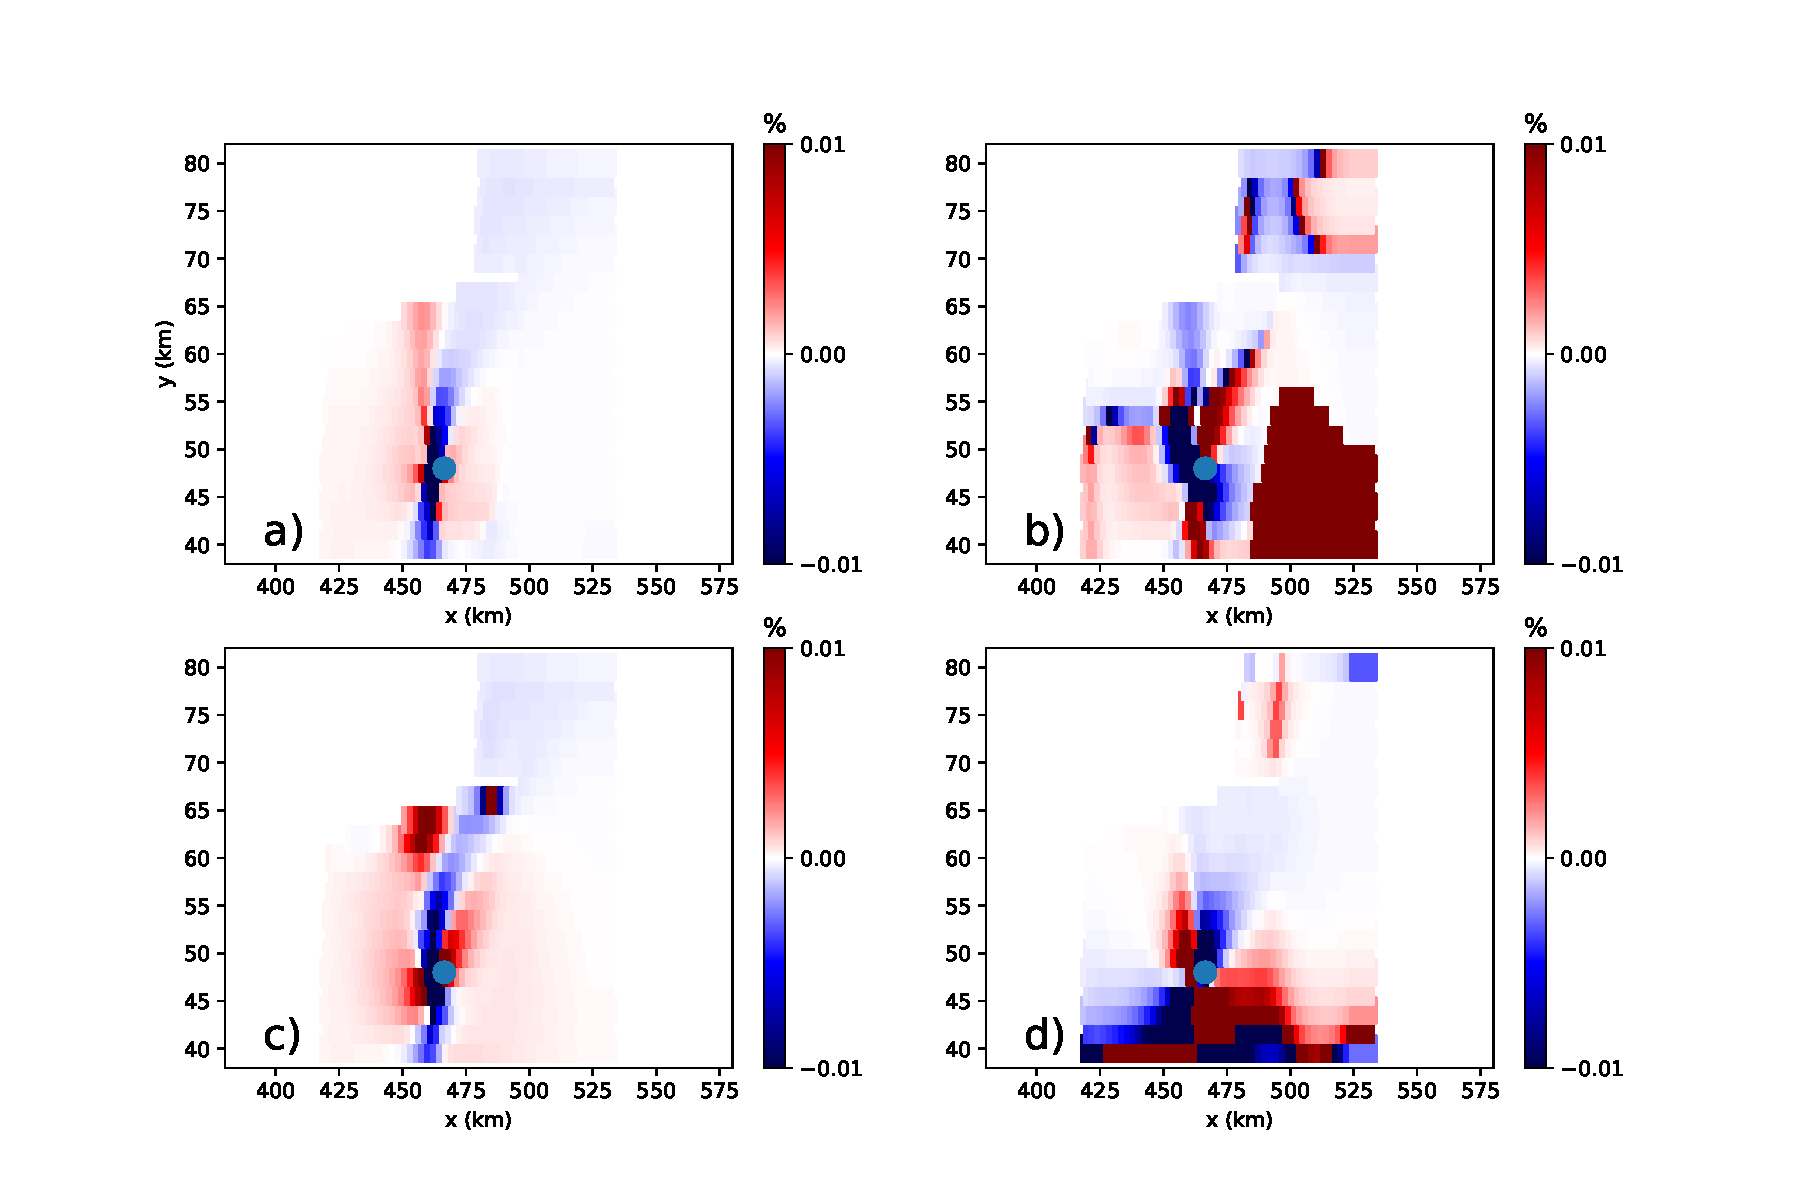
\includegraphics[width=1\linewidth]{figs/stressDiff.pdf}
%	\caption{An example of stress component changes (\%) across the MISMIP+ ice shelf and grounding line after apply the perturbations at different locations (blue circles). (a) Changes of $\sigma_{p1}$; (b) Changes of $\sigma_{p2}$; (c) Changes of $\sigma_{f}$; (d) Changes of $\sigma_{s}$;.}
%	\label{stressDiff}
%\end{figure}
%
%\begin{figure}
%	\centering
%	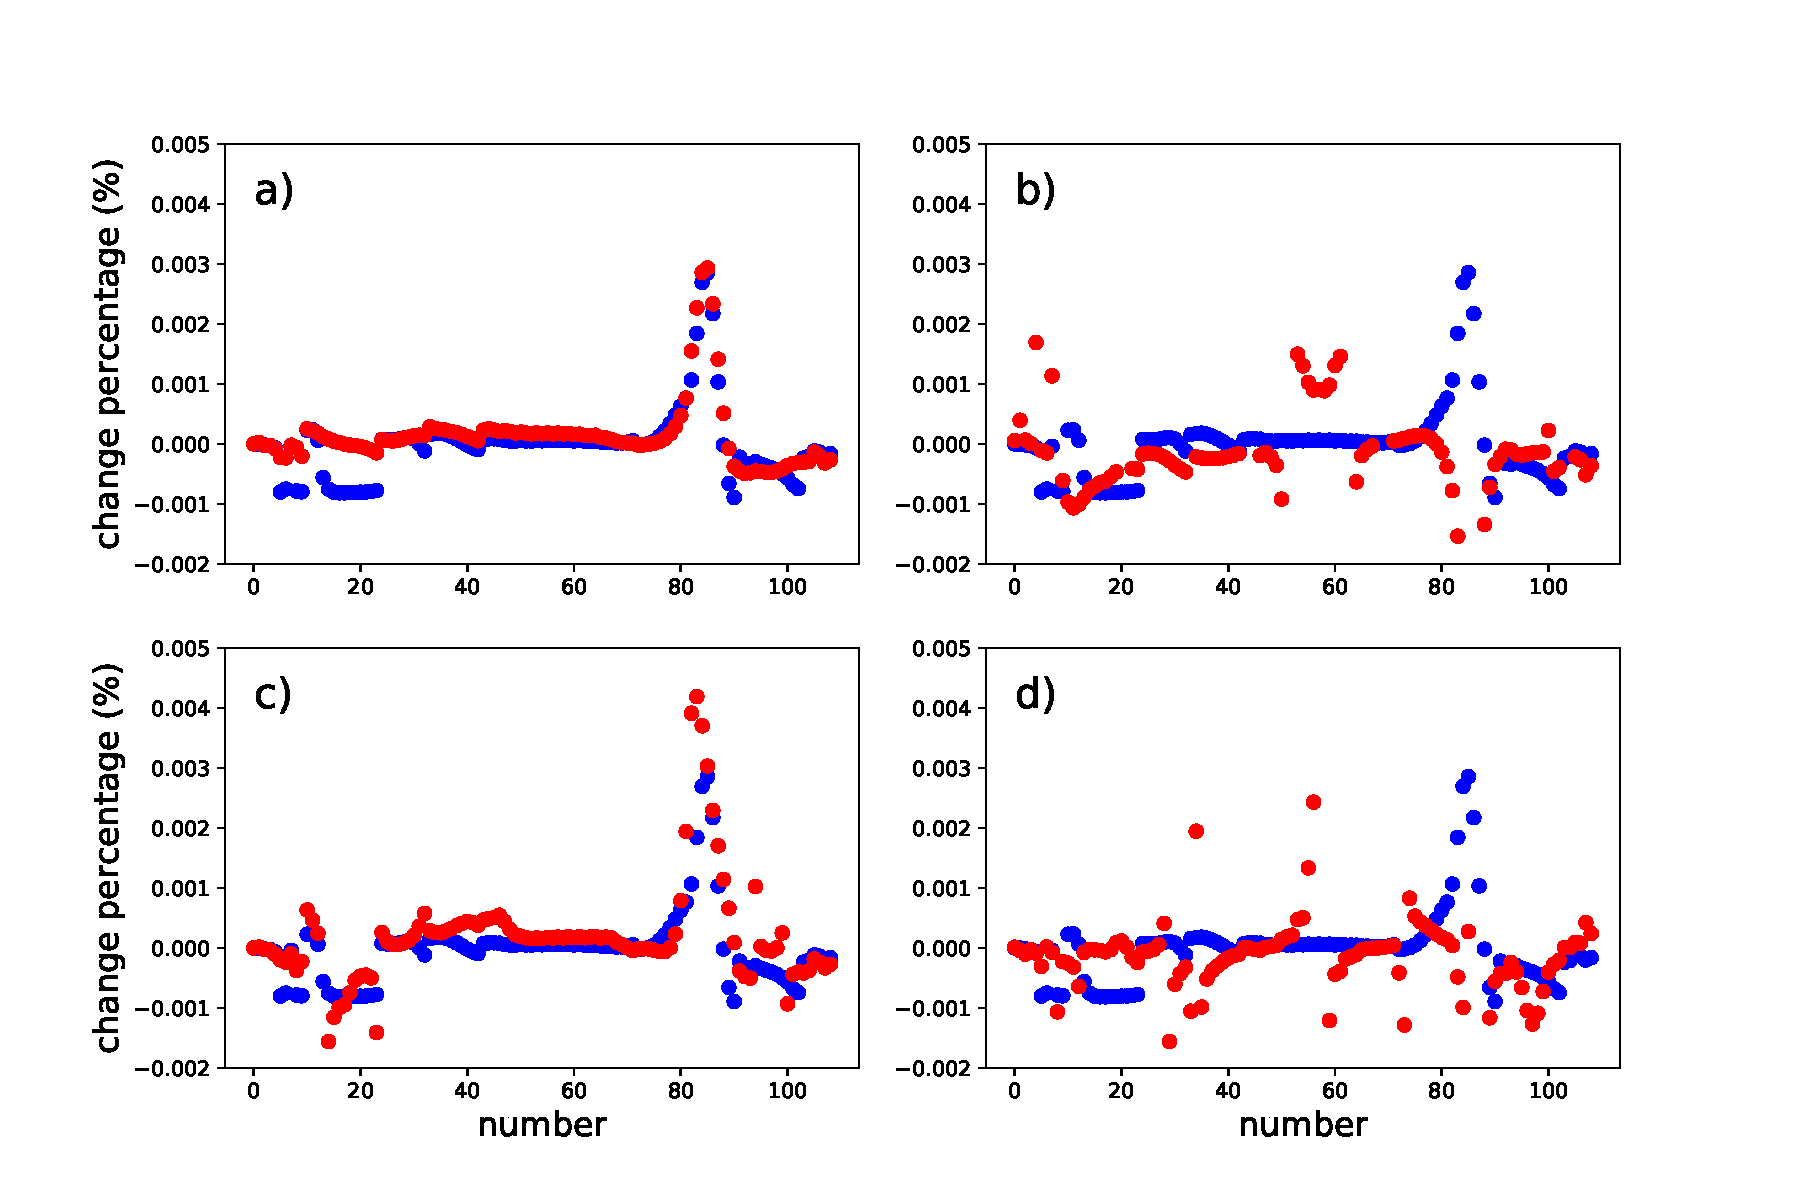
\includegraphics[width=1\linewidth]{figs/diffStress_diffVel.pdf}
%	\caption{The change percentage of ice speed (blue dots) and stress components (red dots; a--d represents $\sigma_{p1}$, $\sigma_{p2}$, $\sigma_{f}$ and $\sigma_{s}$, respectively) for all cells at the grounding line corresponding to Fig.~\ref{stressDiff}.}
%	\label{stressDiff_velDiff}
%\end{figure}

\end{document}
